\section{LLaDA2.0 Training Paradigm}

\begin{figure}
    \centering
    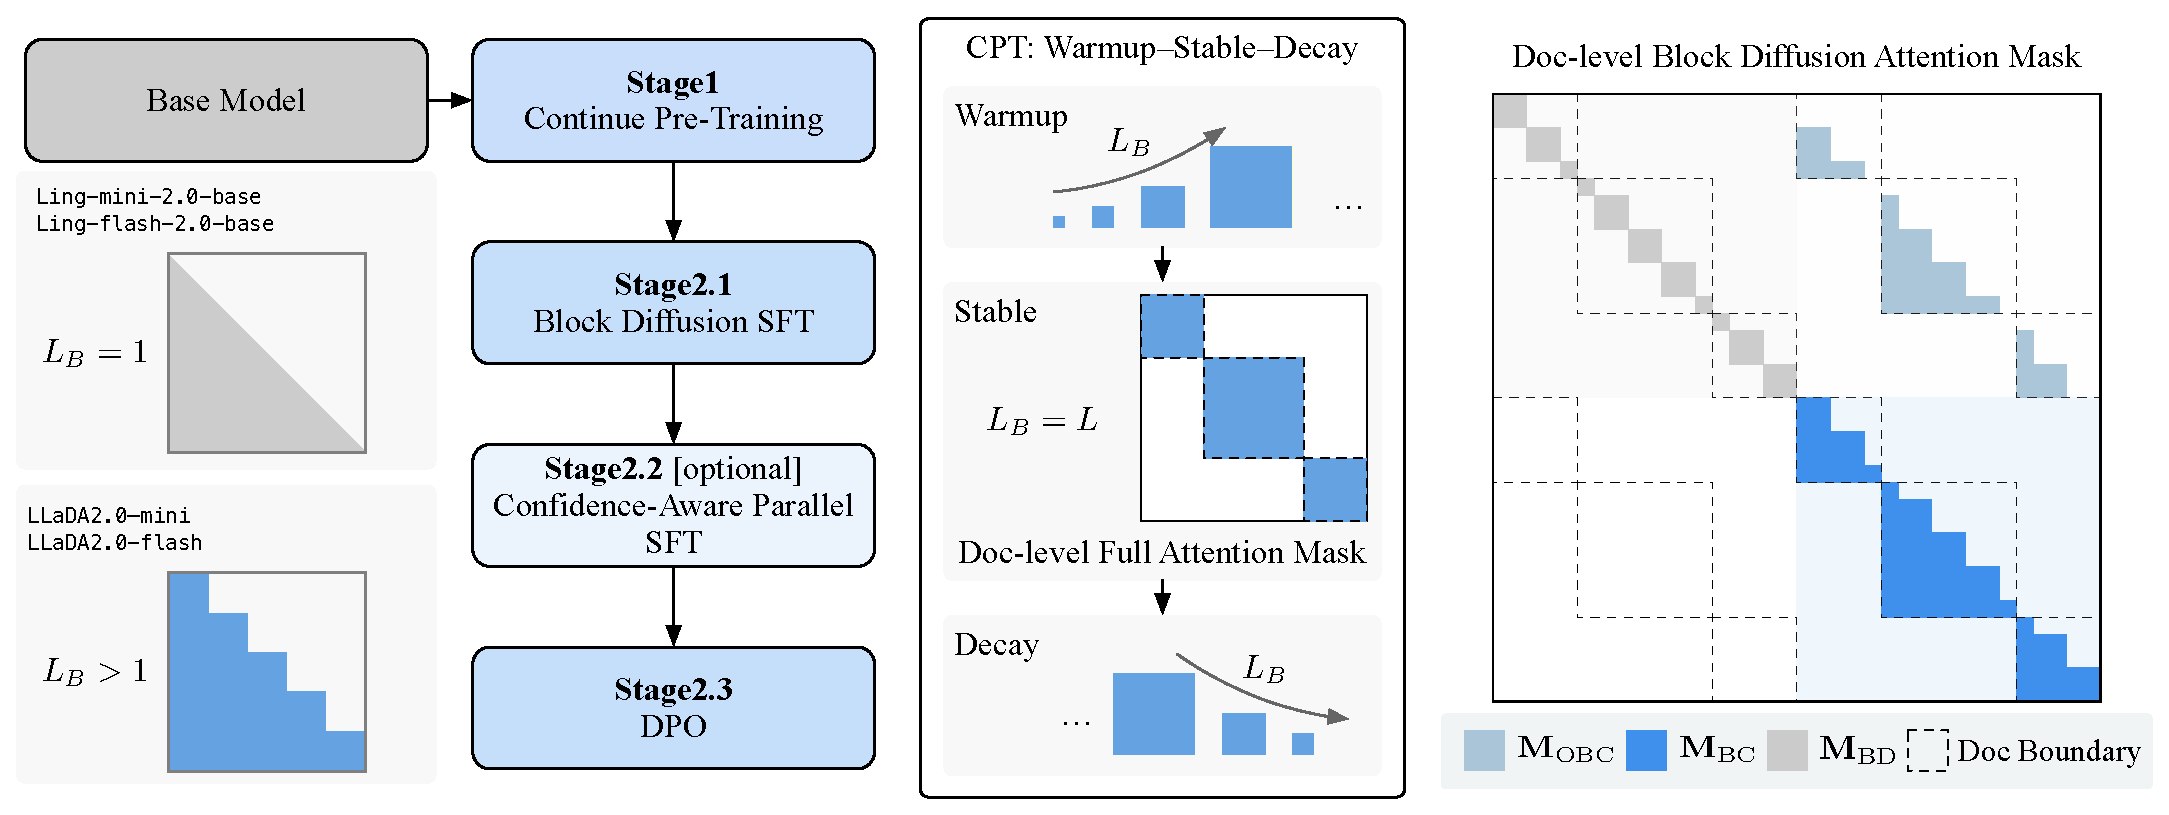
\includegraphics[width=\linewidth]{images/AR2MDLM-pipeline-v2}
    \caption{\textbf{A schematic of the progressive training framework for transforming an AR model into a MDLM.} Continual Pre-Training Stage facilitates the \textbf{Warmup-Stable-Decay} strategies by scheduling block size $L_{B}$ enables smooth, stable, and effective attention mask adaptation. Post-training Stage facilitates the same block diffusion configuration conducting the instruction SFT, Confidence-Aware Parallel SFT, and DPO. The right panel illustrates the document-level block diffusion attention mask,which enables an efficient, vectorized forward pass by constructing a single input sequence from multiple noisy and clean examples, such as $[\bm{x}_{\text{noisy1}},\dots,\bm{x}_{\text{clean1}},\dots]$. The forward pass then employs a combination of block-diagonal ($\mathbf{M}_{\text{BD}}$), offset block-causal ($\mathbf{M}_{\text{OBC}}$), and block-causal ($\mathbf{M}_{\text{BC}}$) masks.}
    \label{fig:llada2_paradigm}
\end{figure}

Figure~(\ref{fig:llada2_paradigm}) illustrates the holistic training pipeline of LLaDA2.0, a staged and scalable framework designed to transform AR language models into highly efficient diffusion language models. Our paradigm follows a three-stage progression: (1) \textit{Continual Pre-training} from AR to MDLM, (2) \textit{Block Diffusion Pre-training} to transition from token-level to block-level diffusion modeling, and (3) \textit{Post-training} for alignment and task specialization.

The process begins with a strong AR base model. We first perform continual pre-training to adapt this model into an MDLM, where it learns to reconstruct randomly masked tokens in a bidirectional, denoising fashion. This phase bridges the gap between AR and diffusion-based generation while preserving the representational geometry of the original model.

Building upon the trained MDLM, we then introduce \textit{block diffusion pre-training}, during which the model is further trained to denoise contiguous spans of text—referred to as “blocks”—rather than individual tokens. This shift enables higher computational efficiency and better long-range coherence during generation.

Finally, after mastering non-autoregressive generation at both token and block levels, the model undergoes post-training--including SFT and DPO to align its outputs with human intent, instruction-following capability, and downstream application requirements. This stage ensures that the powerful generative backbone developed during diffusion pre-training translates into practical performance gains across diverse tasks.


Overall, LLaDA2.0’s training paradigm emphasizes \textbf{knowledge inheritance}, \textbf{progressive adaptation}, and \textbf{efficiency-aware design}, enabling seamless evolution from AR models to fluent, flexible, and fast diffusion large language models.
